\documentclass{article}

% Language setting
% Replace `english' with e.g. `spanish' to change the document language
\usepackage[portuguese]{babel}

% Set page size and margins
% Replace `letterpaper' with `a4paper' for UK/EU standard size
\usepackage[a4paper,top=2cm,bottom=2cm,left=3cm,right=3cm,marginparwidth=1.75cm]{geometry}

% Useful packages
\usepackage{amsmath}
\usepackage{subcaption}
\usepackage{graphicx}
\usepackage[colorlinks=true, allcolors=blue]{hyperref}

\title{Trabalho Prático 05}
\author{Luciano Stork}

\begin{document}
\maketitle

\begin{abstract}
Chegando ao último trabalho prático referente à disciplina, dessa vez foi proposta uma abordagem sobre a utilização do código de Hamming para detecção e correção de erros. Vale citar, nesse cenário, a importância dessa metodologia de implementação no campo das comunicações e na transmissão de dados. O código de Hamming é uma técnica crucial para assegurar a integridade das informações em sistemas de comunicação.

No âmbito das telecomunicações, onde a transmissão de dados é suscetível a interferências e ruídos, a aplicação do código de Hamming se destaca por sua capacidade não apenas de identificar erros, mas também de corrigi-los de maneira eficiente. Essa propriedade o torna uma ferramenta valiosa em ambientes onde a precisão na transmissão de dados é fundamental, como em sistemas de comunicação digital e armazenamento de informações.

Ao explorar essa técnica, é possível compreender como os bits de paridade são estrategicamente introduzidos na mensagem original, permitindo a detecção e, em alguns casos, a correção de erros ocorridos durante a transmissão. Dessa forma, o código de Hamming contribui não apenas para a confiabilidade, mas também para a eficiência dos sistemas de comunicação, promovendo a entrega de informações precisas e íntegras.

Ao longo desta atividade prática, a imersão nos detalhes da implementação do código de Hamming permitirá uma análise aprofundada dos mecanismos práticos subjacentes a essa poderosa ferramenta de detecção e correção de erros. Explorar uma variedade de casos de teste proporcionará uma compreensão mais ampla da versatilidade do algoritmo, revelando como ele responde a diferentes padrões de dados e condições de transmissão.

Esta experiência prática transcende a mera consolidação do conhecimento teórico adquirido em sala de aula, fornecendo uma perspectiva dinâmica e aplicada dos conceitos fundamentais da teoria da informação. Ao enfrentar desafios reais na manipulação e transmissão de dados, torna-se possível não apenas solidificar a compreensão teórica, mas também ganhar insights valiosos sobre a complexidade e as nuances envolvidas na prática da codificação de Hamming.

Cito que foi inicialmente sugerida a abordagem deste projeto com base na utilização da função 'hammgen', responsável por gerar  os bits de paridade de acordo com o código de Hamming. No entanto, em oportunidades de conversas com o professor na última aula (20/11/2023), o mesmo sugeriu que utilizássemos a função 'encode' com o parâmetro 'hamming' configurado. Deste modo, além de uma implementação significativamente mais tranquila, essa abordagem agrega mais agilidade ao processo. Portanto, para a confecção da parte prática desse trabalho, utilizo a função nativa previamente explorada de forma recursiva, adaptando-a a cada dado de entrada.

\end{abstract}

\section{Introduzindo os conceitos}

Para iniciar, de fato, a implementação do código, é interessante conhecer minimamente como funciona a abordagem aqui desenvolvida. O código de Hamming é uma técnica de detecção e correção de erros em transmissões de dados, desenvolvida pelo matemático Richard Hamming. Sua principal função é assegurar a integridade da informação em ambientes sujeitos a interferências, ruídos e potenciais erros de transmissão. Esse método se destaca pela sua capacidade não apenas de identificar, mas também de corrigir erros, proporcionando maior confiabilidade em sistemas de comunicação.

Ao implementar o código de Hamming, bits de paridade são estrategicamente introduzidos na mensagem original. Esses bits extras servem como "verificadores" que permitem detectar se ocorreu algum erro durante a transmissão. Além disso, em casos em que um erro é identificado, o código de Hamming é projetado para corrigi-lo, garantindo a precisão dos dados.

O processo de atribuição de bits de paridade no código de Hamming é conduzido de maneira sistemática e estratégica, visando oferecer tanto detecção quanto correção de erros. Inicialmente, ao considerar uma mensagem original de \( k \) bits, \( r \) bits de paridade são adicionados, com \( 2^r \) sendo maior ou igual a \( k + r + 1 \). Essa condição é essencial para garantir que os bits de paridade possam cobrir todos os bits da mensagem, incluindo eles próprios.

A alocação dos bits de paridade segue uma lógica específica, sendo posicionados em lugares correspondentes a potências de 2. Essa disposição facilita o cálculo dos bits de paridade e a identificação eficiente de erros. Em termos de cálculo, cada bit de paridade é responsável por verificar um conjunto específico de bits na mensagem, utilizando a operação lógica XOR (\(\oplus\)) para garantir que a soma dos bits verificados seja sempre par.

Após o cálculo, os bits de paridade são incorporados à mensagem original nos locais designados, resultando em uma mensagem expandida. Essa mensagem, agora contendo bits de paridade, é então transmitida ou armazenada. Esses bits adicionais desempenham um papel crucial na detecção e, em alguns casos, correção de erros durante a recuperação da informação.

Ao receber a mensagem, o destinatário recalcula os bits de paridade utilizando os dados recebidos. Caso um erro tenha ocorrido durante a transmissão, a posição do bit de paridade com erro permite identificar o bit problemático. Em algumas situações, a correção é possível, proporcionando uma maior confiabilidade no processo de comunicação.

Um exemplo prático de utilização do código de Hamming está em sistemas de memória de computadores. Em ambientes onde a integridade dos dados é crucial, como em módulos de RAM, onde o código de Hamming é frequentemente empregado. Se um bit for corrompido durante a leitura da memória, o código de Hamming pode identificar e corrigir automaticamente o erro, assegurando que os dados armazenados sejam confiáveis.

Outra aplicação comum está na transmissão de dados em redes de comunicação, especialmente em canais suscetíveis a interferências. Em sistemas de comunicação digital, o código de Hamming garante que a informação transmitida seja recebida de forma precisa, mesmo em ambientes propensos a ruídos.

Nesse sentido, torna-se importante ressaltar que o código de Hamming, embora eficiente na detecção e correção de erros isolados, possui limitações, especialmente em relação a erros múltiplos ou padrões específicos que podem não ser corrigidos de maneira eficiente. No entanto, sua aplicação estratégica faz dele uma ferramenta valiosa em ambientes onde a precisão e a confiabilidade na transmissão de dados são fundamentais.

\section{Implementação do algoritmo}
\subsection{Entendendo a abordagem}
Como citado, inicialmente foi sugerido pelo professor a utilização da função “hammgen” para gerar os bits de paridade de acordo com o código de Hamming, sendo o algoritmo capaz de receber uma sequência de dados binários como entrada, adicionar os bits de paridade e gerar a sequência de dados codificados. 

Entretanto, na aula presencial do dia 20/11/2023, descobrimos, juntamente com o professor, uma função que encapsula todo o processo de codificação de Hamming. Trata-se do comando \textbf{encode}, que é um codificador de bloco nativo no Matlab. Essa função desempenha um papel central na implementação de técnicas de controle de erro, como o código de Hamming.

Ela aceita como entrada a mensagem binária (\textbf{MSG}), o tamanho total do código resultante (\textbf{N}), o número de bits de mensagem (\textbf{K}), o método de codificação (\textbf{METHOD}), e opções adicionais específicas para o método escolhido (\textbf{OPT}). No presente caso, utilizo o comando \textbf{encode 'hamming'} e a função implementa automaticamente o código de Hamming, adicionando bits de paridade à mensagem para detecção e, em alguns casos, correção de erros. 

Tal utilização se revelou valiosa, simplificando significativamente a implementação do código de Hamming no projeto e proporcionando uma solução integrada e eficiente para aplicações de controle de erro no âmbito da teoria da informação, encapsulando o esforço para gerar uma lógica que fizesse de forma manual as etapas da codificação em análise.

\subsection{Etapa de Codificação}
Na etapa de codificação por Hamming em si, penso em abordar o problema de forma recursiva. Então, inicio o código limpando o buffer e fechando as demais aplicações e janelas com os comandos \textbf{close all}, \textbf{clear} e \textbf{clc}. Em seguida, forneço uma mensagem binária de entrada e calculo seu tamanho. Essa informação do tamanho da mensagem binária se faz importante tanto na chamada da função propriamente dita, quanto na contribuição para determinar o número de bits de paridade necessários para a implementação.

Desse modo, prossigo no código criando um loop que vai ser responsável por obter, a partir da mensagem inserida, a quantidade de bits de paridade necessária, agregando certa iteratividade ao código, tornando-o adaptativo à entrada de dados. Assim sendo, O loop é iniciado e a condição \(2^{num\_bits\_parity} < num\_bits\_dados + num\_bits\_parity + 1\) garante que o número de bits de paridade seja suficiente para cobrir tanto os bits de dados quanto os bits de paridade, conforme requerido por certas técnicas de codificação. Dentro do loop, o número de bits de paridade (\textit{num\_bits\_parity}) é incrementado em 1 a cada iteração, até que a quantidade necessária seja alcançada. 

Após finalizar o laço for e obter a quantidade de bits de paridade necessários, obtenho o tamanho total da palavra, com a operação de soma da quantidade de bits de dados mais a quantidade de bits de paridade. Essa seria outra informação pertinente na chamada da função.

A seguir, utilizo a função \textbf{encode}, com os dados de entrada \textbf{palavra} (que seria a sequência binária de entrada), \textbf{tam\_total} (tamanho da palavra + quantidade de bits de paridade), \textbf{num\_bits\_dados} (quantidade de elementos da palavra binária), \textbf{'hamming'} (método de codificação utilizado). E então é gerada a codificação Hamming da palavra binária original.

Para a decodificação, utilizo a função \textbf{decode} seguindo a mesma lógica. Altero apenas a entrada \textbf{palavra} por \textbf{code} e obtenho a palavra binária original como saída.

Posteriormente, introduzi erros artificiais na transmissão, simulando condições adversas. Especificamente, nas posições dos bits 2 e 5, identificadas pelo vetor \textbf{pos\_erros}. Isso foi realizado através da criação de uma cópia da palavra codificada original (\textbf{code}) denominada \textbf{code\_erro}. Os bits nessas posições foram invertidos utilizando a operação lógica de negação (\textbf{~}). Este processo simula possíveis erros que podem ocorrer durante a transmissão.

Em seguida, a palavra codificada com os erros introduzidos (\textbf{code\_erro}) foi também submetida à função \textbf{decode}. Esta função, utilizando o método de Hamming, tem como resultado a obtenção da mensagem decodificada. Este passo é crucial para avaliar a capacidade do código de Hamming em detectar e corrigir erros, contribuindo para a confiabilidade da transmissão de dados.

Finalizo o programa apresentando os resultados de forma sistemática, exibindo a palavra original, a codificação e decodificação. Em um primeiro momento, sem erros na transmissão, revelo a sequência binária original e sua respectiva codificação Hamming. Posteriormente, introduzo erros artificiais nas posições específicas, simulando condições adversas na transmissão. Nesse contexto, exibo a palavra codificada com erros. Concluo a apresentação mostrando a decodificação da palavra, evidenciando a capacidade do código de Hamming em detectar e corrigir esses erros, contribuindo para a confiabilidade da transmissão de dados.


\section{Análise dos resultados obtidos}
Noto que a função \textbf{encode} não codifica tão corretamente os bits de paridade esperados para as sequências binárias sob a lógica de Hamming; obtendo, nos resultados dos testes, palavras codificadas inusitadas. O motivo pelo qual chego a essa conclusão está baseado na comparação das palavras formadas no algoritmo e dos resultados de calculadora de Hamming, como por exemplo a disponível em \href{http://www.mathaddict.net/hamming.htm}{link para a calculadora de Hamming}. 

Para exemplificar essa ideia, disponibilizo os testes no algoritmo seguidos das comparações na calculadora, explícitos nas seguintes imagens:

\begin{figure}[htbp]
    \centering
    \begin{subfigure}[b]{0.22\textwidth}
        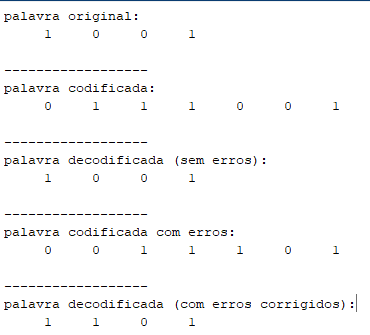
\includegraphics[width=\textwidth]{4bitsCaso01.png}
        \caption{Caso 01: 1001}
        \label{fig:imagem1}
    \end{subfigure}
    \hfill
    \begin{subfigure}[b]{0.22\textwidth}
        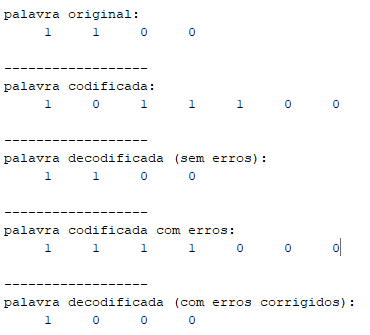
\includegraphics[width=\textwidth]{4bitsCaso02.png}
        \caption{Caso 02: 1100}
        \label{fig:imagem2}
    \end{subfigure}
    \hfill
    \begin{subfigure}[b]{0.22\textwidth}
        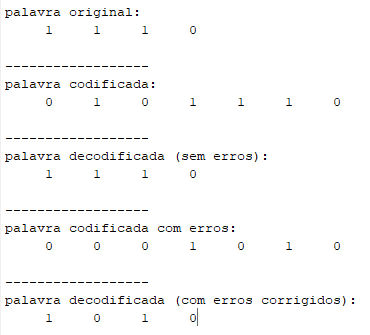
\includegraphics[width=\textwidth]{4bitsCaso03.png}
        \caption{Caso 03: 1110}
        \label{fig:imagem3}
    \end{subfigure}
    \hfill
    \begin{subfigure}[b]{0.22\textwidth}
        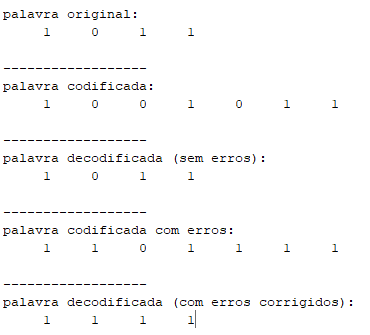
\includegraphics[width=\textwidth]{4bitsCaso04.png}
        \caption{Caso 04: 1011}
        \label{fig:imagem4}
    \end{subfigure}
    
    \caption{Resultados da Função \textbf{encode}}
    \label{fig:conjunto-imagens}
\end{figure}

\afterpage{\clearpage}

\begin{figure}[htbp]
    \centering
    \begin{subfigure}[b]{0.22\textwidth}
        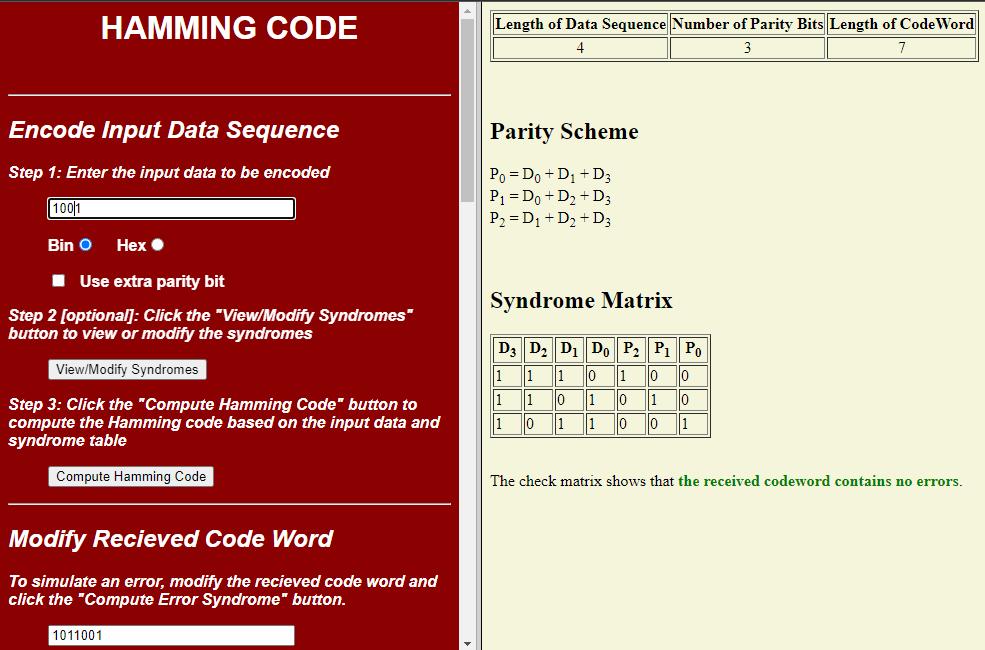
\includegraphics[width=\textwidth]{4bitsCaso01_Calculadora.png}
        \caption{Calculadora Caso 01: 1001}
        \label{fig:imagem1}
    \end{subfigure}
    \hfill
    \begin{subfigure}[b]{0.22\textwidth}
        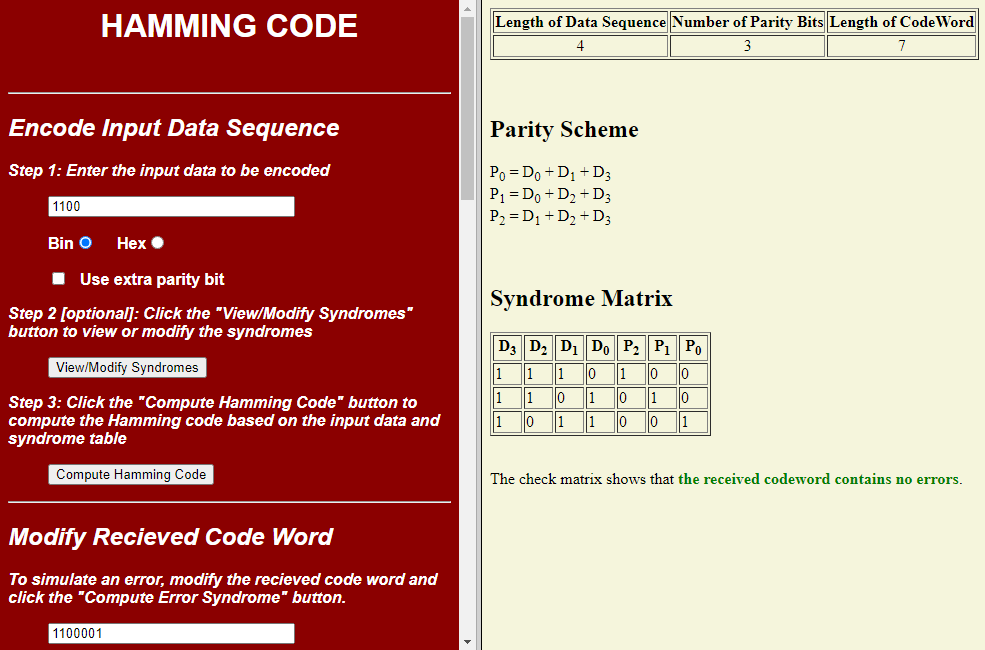
\includegraphics[width=\textwidth]{4bitsCaso02_Calculadora.png}
        \caption{Calculadora Caso 02: 1100}
        \label{fig:imagem2}
    \end{subfigure}
    \hfill
    \begin{subfigure}[b]{0.22\textwidth}
        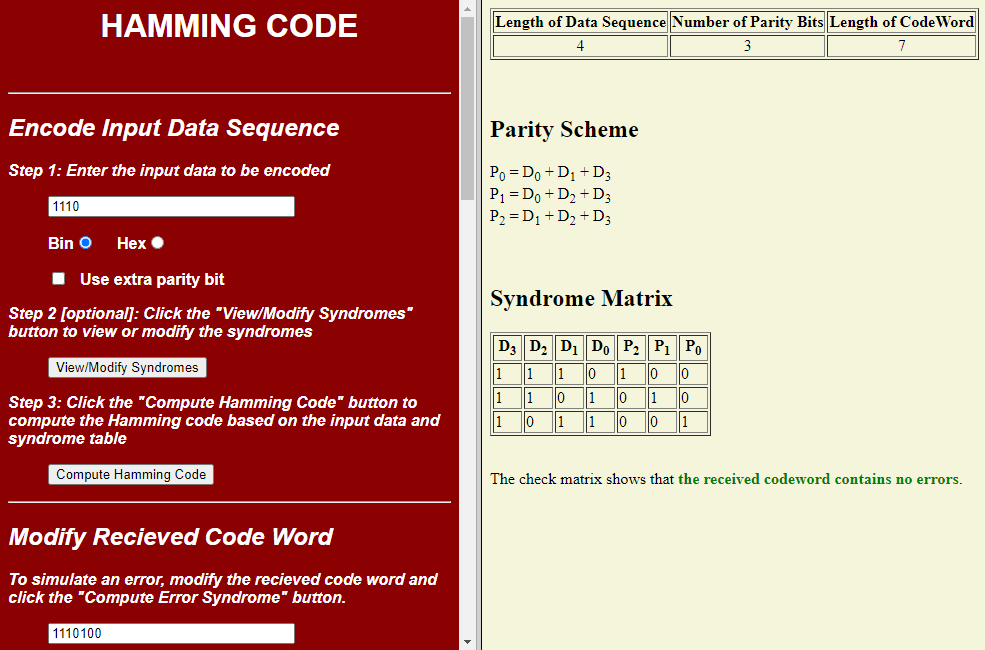
\includegraphics[width=\textwidth]{4bitsCaso03_Calculadora.png}
        \caption{Calculadora Caso 03: 1110}
        \label{fig:imagem3}
    \end{subfigure}
    \hfill
    \begin{subfigure}[b]{0.22\textwidth}
        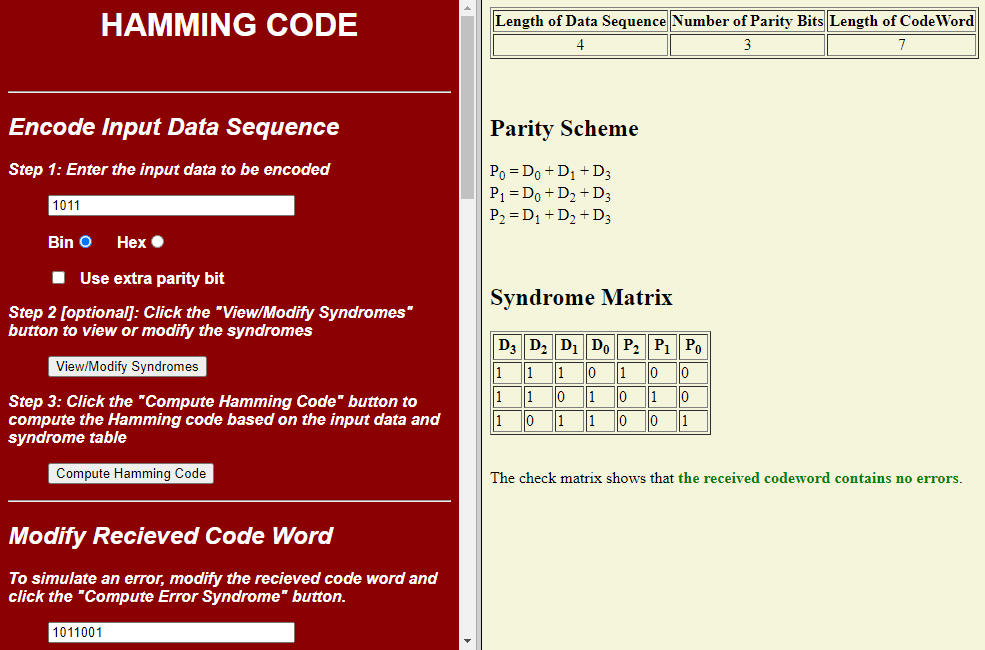
\includegraphics[width=\textwidth]{4bitsCaso04_Calculadora.png}
        \caption{Calculadora Caso 04: 1011}
        \label{fig:imagem4}
    \end{subfigure}
    
    \caption{Resultados da Calculadora de Hamming}
    \label{fig:conjunto-imagens}
\end{figure}

Portanto, com base nessa análise, acredito que a função \textbf{encode} para o método \textbf{'hamming'} ou não está bem definida no Matlab, ou não fornece a lógica correta para o resultado esperado.

Um ponto interessante é que ela limita o tamanho da palavra binária para os casos típicos da codificação de Hamming. Isto é, a função aceita somente as entradas compatíveis com as entradas mais conhecidas das codificações de Hamming, como a \textbf{(7,4)}, \textbf{(15,11)} e \textbf{(31,26)}, por exemplo.

Além disso, percebo que o mecanismo de correção para a adição de erros artificiais não se mostrou totalmente eficiente; não recuperando, por vezes, a sequência binária original de forma satisfatória.

Menciono, por fim, que, por característica da tecnologia, a codificação de Hamming, embora eficaz na detecção e correção de erros em palavras de código, possui a capacidade de detecção vinculada a um número específico de bits incorretos na palavra de código, e se esse número exceder sua capacidade de correção, a detecção ocorrerá, mas a correção será impossível. A dependência de um padrão específico de bits e a introdução de redundâncias, essenciais para a eficiência do método, contribuem para um aumento na largura de banda necessária, limitando sua aplicabilidade em contextos com restrições de recursos computacionais.

A complexidade de implementação da codificação de Hamming cresce proporcionalmente ao número de bits na palavra de código, podendo ser uma consideração significativa em sistemas com recursos limitados. Além disso, a eficácia do método diminui em face de erros múltiplos na mesma palavra de código, e a presença de ruídos transitórios pode desafiar sua correção, sendo mais eficaz contra erros permanentes. Considerar as limitações específicas em diferentes aplicações é crucial, e em ambientes com latências extremamente baixas, a sobrecarga introduzida pela codificação de Hamming pode ser uma preocupação relevante. 

Em conclusão, embora seja valiosa em muitos contextos, a escolha de métodos alternativos deve ser ponderada cuidadosamente de acordo com os requisitos específicos de cada aplicação.


\bibliographystyle{alpha}
\bibliography{sample}
\begin{enumerate}
    \item 
    Material disponibilizado pelo professor Leonardo Carneiro como suporte à disciplina Teoria da Informação e Codificação 
    \item 
    http://www.mathaddict.net/hamming.htm
    \item https://www.dcode.fr/hamming-error-correction?\_\_r=1.ba79dabf92f910f7962bc68ce2ec2b81
    \item https://pt.wikipedia.org/wiki/C%C3%B3digo\_de\_Hamming
    \item https://www.ime.usp.br/~song/mac412/hamming.pdf
\end{enumerate}
\end{document}